\documentclass[journal]{IEEEtran}

\usepackage{graphicx}          %graph
\usepackage[backref]{hyperref} %reference
\usepackage{float}    %format H
\usepackage{amsmath}  %equation
\usepackage{multirow} %table multirow 


\hyphenation{op-tical net-works semi-conduc-tor}


\begin{document}

\title{Face Image Inpainting with Evolutionary Generators}

\author{Chong~Han,~\IEEEmembership{}
        Junli~Wang~\IEEEmembership{}
\thanks{Manuscript received July 26, 2020; revised October 2, 2020. This work was supported in part by the National Key R\&D Program of China(2017YFA0700602), in part by the National Natural Science Foundation of China(No.61672381); in part by the Fundamental Research Funds for the Central Universities.(Corresponding author: Junli Wang)}
\thanks{C. Han and J. Wang are with the Department of Electronics and Information Engineering, Tongji University, Shanghai 201804, China(e-mail: 496274966@qq.com; e-mail: junliwang@tongji.edu.cn)}
}

\markboth{IEEE SIGNAL PROCESSING LETTERS,Vol.14, No.3, October 2020}
{Shell \MakeLowercase{\textit{et al.}}: Bare Demo of IEEEtran.cls for IEEE Journals}
\maketitle

\begin{abstract}
Recently, deep learning has become a mainstream method of image inpainting. It can not only restore the image texture, obtain high-level abstract features of images, but also restore semantic images such as human face images. Among these methods, generative adversarial networks(GANs) using autoencoder as the generator have become the promising model for image inpainting. These models implement the end-to-end image inpainting and also generate visually reasonable and clear image structures and textures. However, GANs often have problems with gradient vanishing and model collapse during training, so we propose a Generative Adversarial Network with Evolutionary Generators (EG-GAN) and apply it in face image inpainting. To stabilize the model training process, EG-GAN trains the generator network by evolution, combines two mutation functions as a training objective to update the parameter of generator networks, and produces offspring generators through crossover, using the matcher assists the discriminator to criticize the generated image. Experiments on various face image datasets such as CelebA-HQ and CelebA show that EG-GAN successfully overcomes the gradient vanishing problem, achieves stable and efficient training, and generates visually reasonable images.
\end{abstract}

\begin{IEEEkeywords}
Neuro-evolution, Autoencoder, Generative Adversarial Networks, Face Image Inpainting.
\end{IEEEkeywords}


\IEEEpeerreviewmaketitle



\section{Introduction}

\IEEEPARstart{I}{mage} inpainting is an important task in machine vision, which aims to fill in missing pixels in damaged images. Initially, Pathak et al. proposed an image inpainting model based on an autoencoder: Context Encoder (CE)\cite{pathak2016context}. Because CE is trained by Euclidean distance, which will inevitably lead to the blurred image\cite{yoo2016pixel}. Afterwards,GAN has become one of the most significant research domains because of its various applications in the field of image processing and multi-view works\cite{hu2019multi}\cite{hu2019multimodal}. Therefore, researchers began to use GANs. For example, Raymond et al. proposed semantic image inpainting with deep generative models(SIIGAN)\cite{yeh2017semantic}. However, this model can't accomplish an end-to-end process, so it takes a lot of time to train. To overcome the above problems, Pathak et al. added an adversarial network into the original CE, which is applied to image inpainting.

Neuro-evolution \cite{floreano2008neuroevolution} is a method that uses biological evolution theory or evolutionary computation to generate artificial neural network parameters, structures, and rules. Therefore, deep learning models based on neuro-evolution can be divided into two categories: the first is to optimize the deep learning model by biological evolution theory. For example, Chaoyue Wang et al. proposed EGAN\cite{wang2019evolutionary}. The second is to use evolutionary computing to optimize deep learning models. Evolutionary computing includes: genetic algorithm (GA), genetic programming (GP), evolutionary strategy (ES), and evolutionary programming (EP). For example, Masanori Suganuma et al. proposed the ES-CAE \cite{suganuma2018exploiting} which applies an evolutionary strategy to autoencoder. Moreover, these experiments prove that deep learning models optimized by neuro-evolution are easier to train and possible to generate some skip connections that are difficult to be designed by a human.

In this letter, EG-GAN is inspired by biological evolution. GAN is trained in the way of neuro-evolution and applied to face image inpainting. EG-GAN mainly consists of three parts: generator, discriminator, and matcher. The generator is regarded as an individual in the population, and the network parameters in the generator are optimized by mutation and crossover. The discriminator is utilized to criticize the quality of the entire generated image. But for image inpainting, the image quality of missing regions is the key to determine the performance of the generator, Therefore, the discriminator has certain limitations. To solve this problem, this letter proposes a matcher to assist the discriminator.The contributions of this letter are summarized as follows:

(1) It is proposed to train the generator by evolution and combine two different mutation functions as the objective function to update the parameters in generators, avoiding the gradient vanishing and model collapse. What's more, a crossover is added to explore the commonality in excellent generator models, producing offspring population, so that elite generators will not be lost in the process of mutation.

(2) A matcher is proposed to assist the discriminator in criticizing the generated image. The matcher can learn to obtain the relevance of each component in the image and focus on criticizing the contextual correlation of the generated regions, avoiding discriminators giving high-value feedback to images with wrong correlation, thereby misleading the generator.

(3) EG-GAN achieves high-quality inpainting results on various face image datasets, including CelebA-HQ, CelebA, PubFig, and non-realistic high-definition face datasets generated by StyleGAN. Meanwhile, the quantitative evaluations on PSNR and SSMI are higher than some traditional and recent image inpainting models.

\section{Generative Adversarial Network with Evolutionary Generator}
\subsection{Neuro-evolution}
We train the entire network by neuro-evolution, regarding the generator as an "individual" in the population, the discriminator and matcher as the "environment" where individuals can be selected in. The whole process includes four steps: mutation, evaluation, selection, and crossover.

(1)Mutation:The essence of mutation is two different objective functions: heuristic mutation and minimax mutation\cite{wang2019evolutionary}, which aim to update the parameters in generators after each evaluation by discriminator and matcher. It is defined as:
    \begin{equation}
    M_G^{heuristic}=-\frac{1}{2}E_{G(x)\sim P_g}[log(D(G(X))]
    \end{equation}
    \begin{equation}
    M_G^{minimax}=\frac{1}{2}E_{G(x)\sim P_g}[log(1-D(G(X))]
    \end{equation}
where Pg is the data distribution of generated image, G(x) is the generated image, and D(G(x)) is the output of discriminator.

Unlike traditional GAN models use a single objective function, EG-GAN uses the combination of heuristic mutation and minimax mutation as the generator's objective function ,avoiding gradient vanishing and model collapse to some extent. As shown in Fig.1, it can guide the model to Nash balance, stabilizing the training process.
\begin{figure}[H]
   \centering
   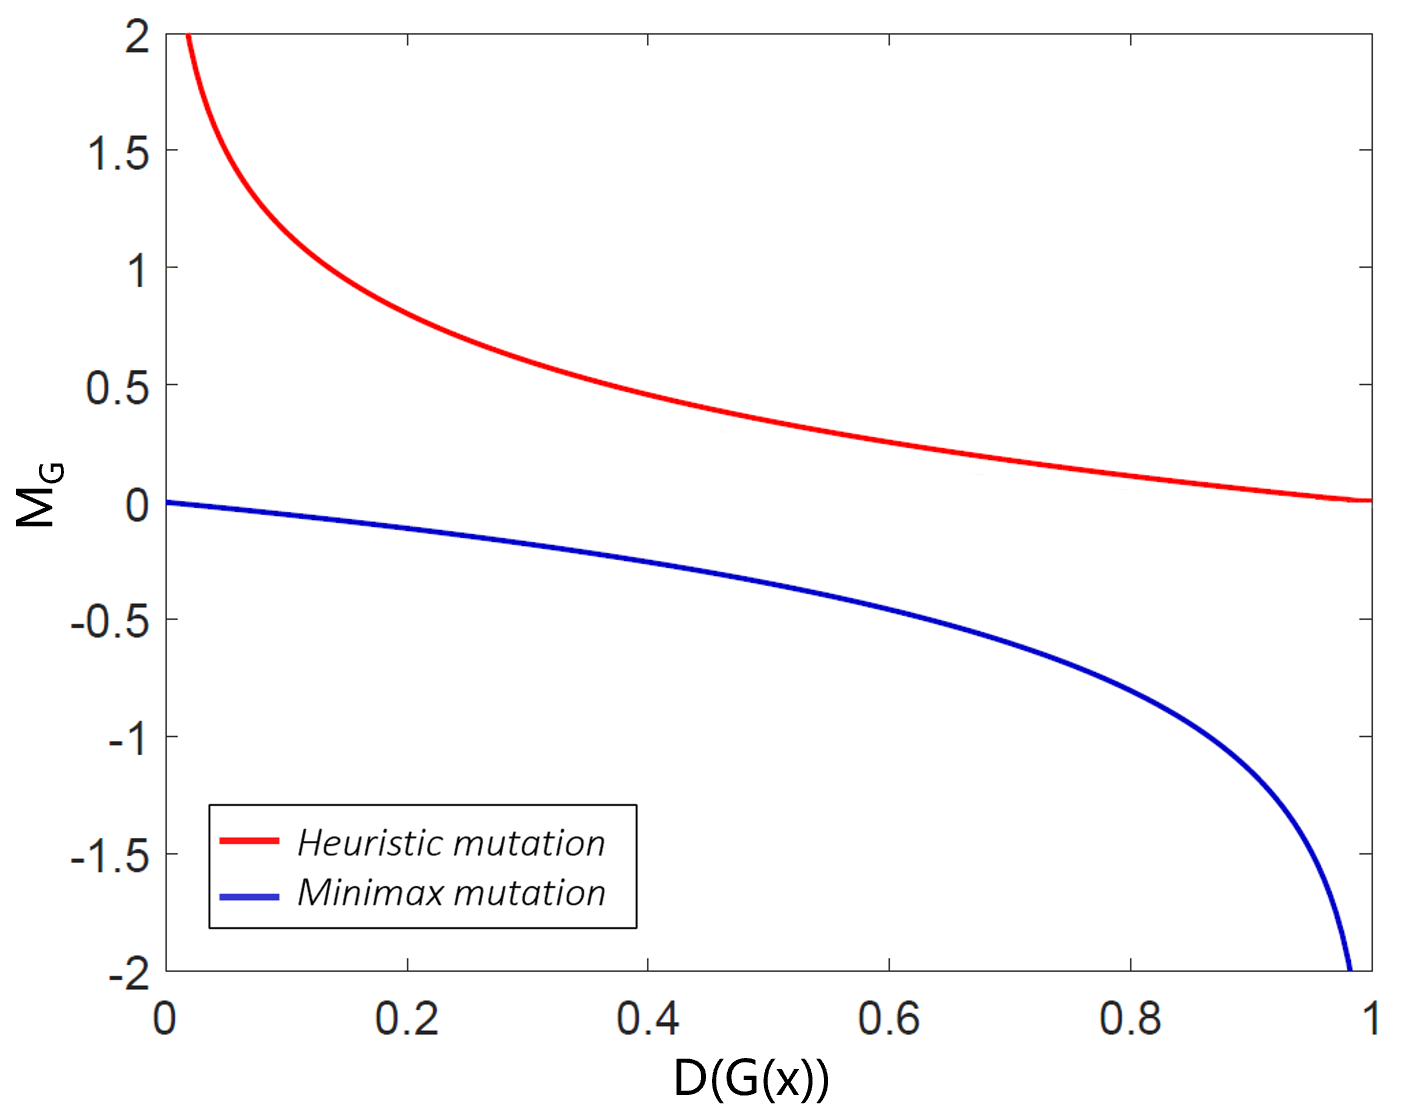
\includegraphics[width=0.6\linewidth]{figures/Fig2.png}
   \caption{Mutation function graph: EG-GAN will determine to use minimax mutation or heuristic mutation: when D(G(x)) is bigger than 0.5, choose the minimax mutation; when D(G(x)) is less than or equal to 0.5, choose the heuristic mutation}
   \label{fig:Fig2}
\end{figure}

(2)Evaluation: In the process of training, using least absolute deviations\cite{de1991l1}(L1loss) as the standard for evaluating the performance of the generators. It reflects the difference between the generated sample and the real sample. It is defined as:
\begin{equation}
L1 = min\sum^n_{i=1} \|x^i-G(x^i)\|
\end{equation}
where x$^{i}$ is a sample from the real data distribution, G(x$^{i}$) is a sample from the generated data distribution, and n is the number of samples.

(3)Selection: According to the value of L1loss, generators will be sorted. Then it will select two generators with the smallest value as a pair of parents and eliminate the rest of individuals. According to the population size, you can keep more than one pair of parents.

(4)Crossover: The generator structure of EG-GAN is encoder-decoder, so the crossover is to produce offspring generators by exchanging the encoder part with each other in a pair of elite parent. In order to avoid the generator's performance fluctuating caused by frequent crossover, the generator executes the crossover only after mutating a certain times(T). The whole process can be seen in the Fig.2
\begin{figure}[H]
\centering
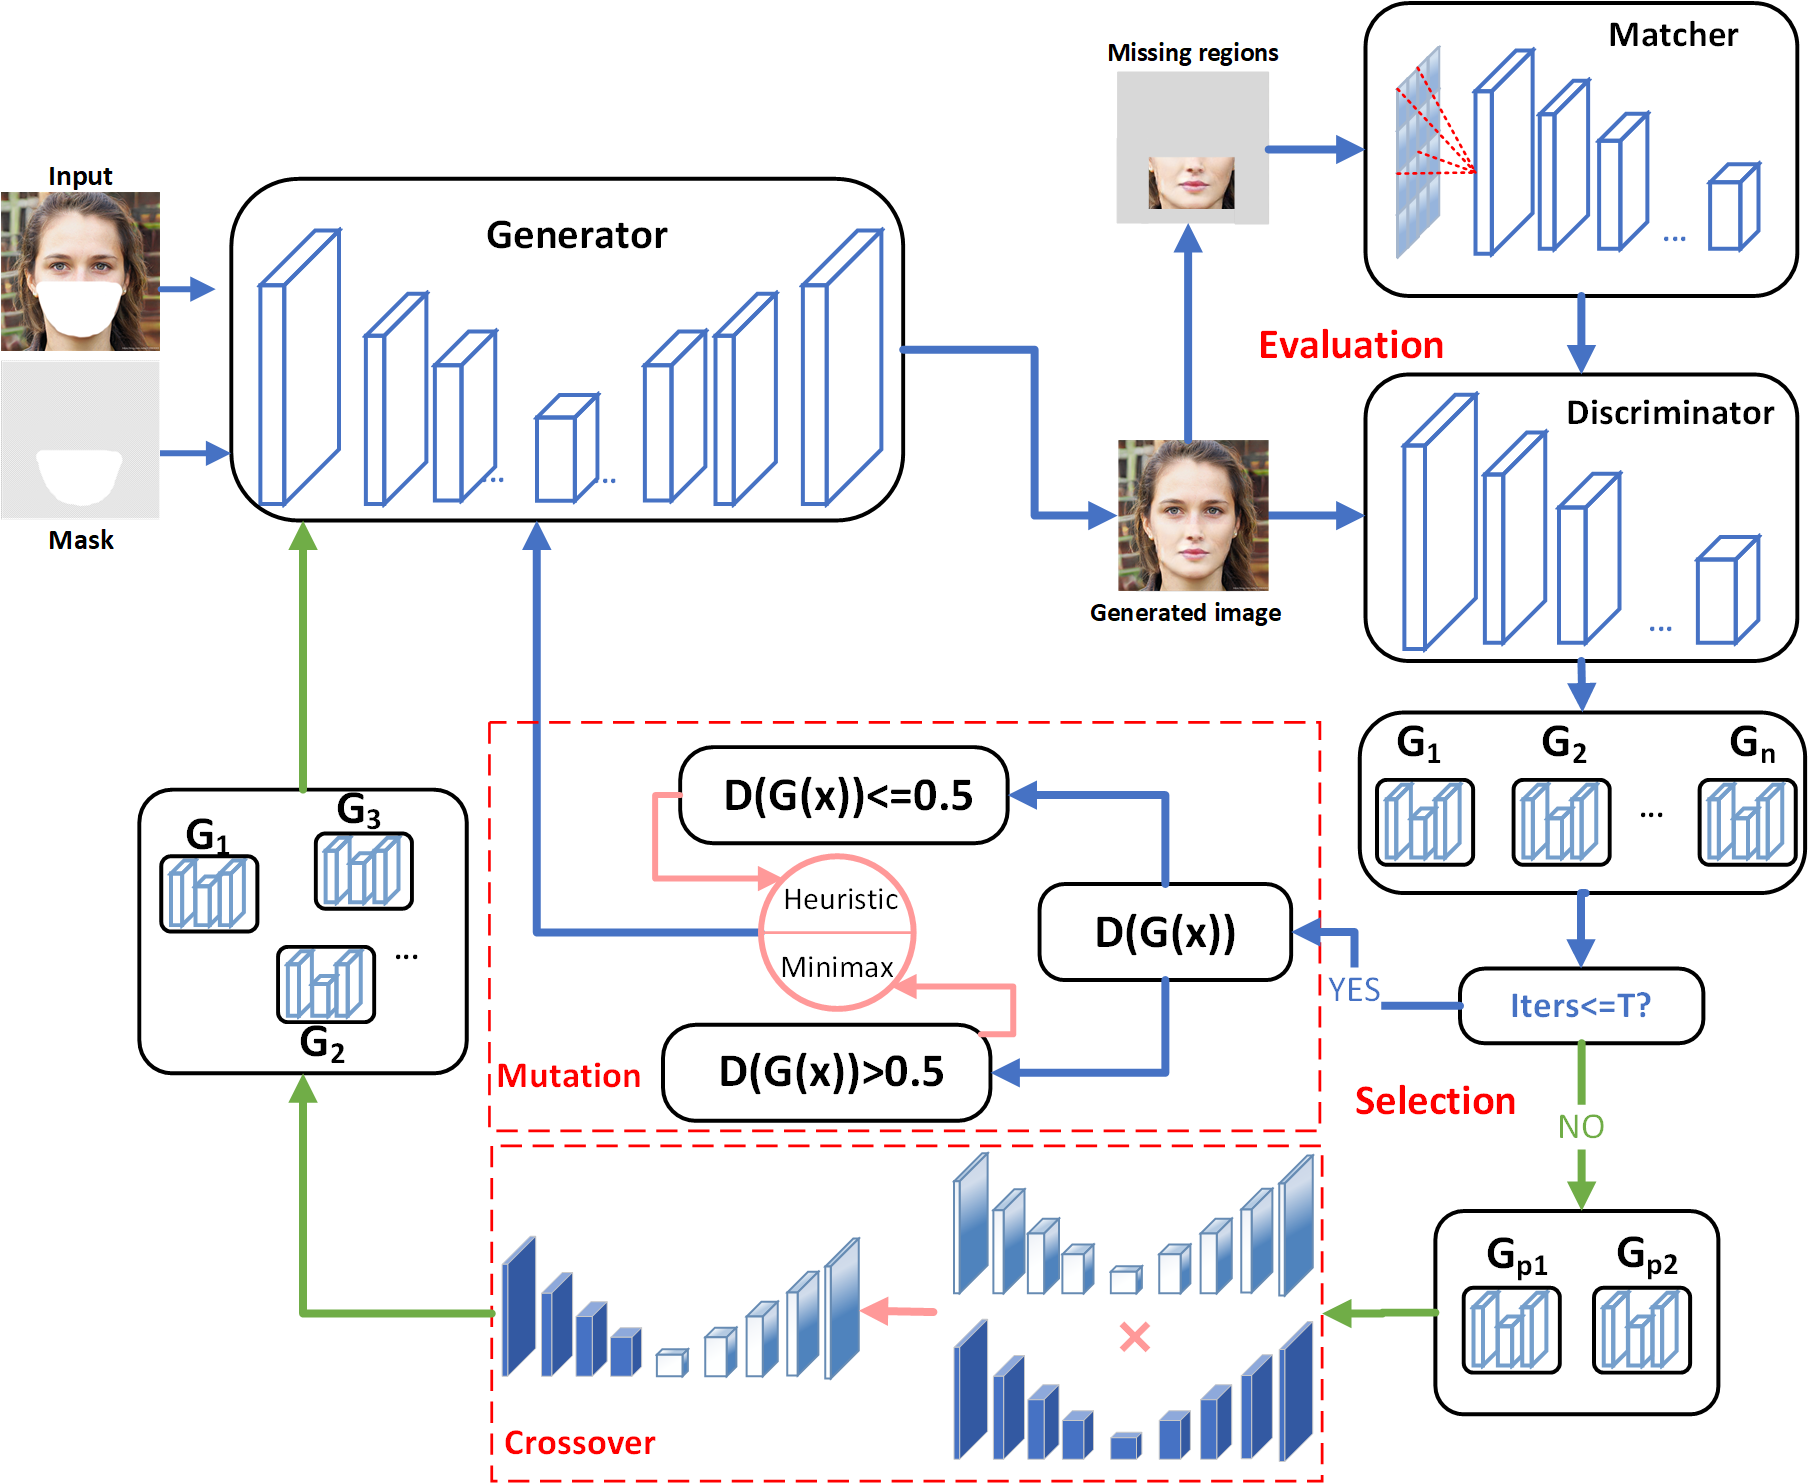
\includegraphics[width=1\linewidth]{figures/Fig1.png}
\caption{EG-GAN framework: The blue line represents the process of updating generator parameters by mutation, and the green line represents the process of producing offspring by crossover.}
\label{fig:Fig1}
\end{figure}
\subsection{EG-GAN}
The generator of our model is autoencoder structure which can directly restore the missing regions of images. The input of the generator is a pair of images. It consists of a damaged face image and a mask (filled by white pixels). The size of the two images is 256 * 256, and the function of the mask is to input the position and shape of the missing regions in images. During training, the face image is blocked by random shapes.

In EG-GAN, the generated images are criticized by two adversarial networks-discriminator and matcher. The discriminator mainly criticizes the authenticity of the entire image, and the matcher focuses on criticizing the authenticity and correlation of missing regions in images.

The input of the matcher is the missing regions of images. The structure of matcher is PatchGAN\cite{isola2017image} to criticize the correlation of generated content. It calculates the pixel differences between the generated image and the original image by the dot product. The result is the loss of the matcher and is also regarded as the penalty of the discriminator. It is defined as formula 4, where m is the mask image, I is the original image.
\begin{equation}
l_m = E_{G(x)\sim P_g}[m\odot D_m(G(x) - I)]
\end{equation}
Discriminator criticizes the authenticity of generated images from a global view to ensure the continuity of the missing boundary pixels. The input of the discriminator is  the complete face image generated by the generators. The network structure is the discriminator in WGAN-GP\cite{gulrajani2017improved}\cite{arjovsky2017wasserstein}. In EG-GAN, the gradient penalty is given by the matcher.

After the generated image is criticized by the matcher and discriminator, the two output values are calculated by weighted summation. Because the authenticity of missing regions is more important, it is defined as formula 5, where $\sigma$ = 0.35 and $\gamma$ = 0.65, D$_{d}$(G(x)) is the output of discriminator,D$_{m}$(G(x)-I) is the output of matcher.

\begin{equation}
D(G(x)) = \sigma D_d(G(x)) + \gamma D_m(G(x)-I)
\end{equation}

According to the penalty provided by the matcher, the discriminator's loss function is defined as formula 6, where D is a 1-Lipschitz function, which meets the conditions of $\|f(x_1)-f(x_2)\|\leq\|x_1 - x_2\|$, so w is a set of 1-Lipschitz functions, P$_{data}$ is the real data distribution. The detailed algorithm can be seen in Fig.3.

\begin{equation}
\begin{aligned}
l_d = &\max_{D\in\omega} \{E_{x \sim P_{data}}[D(x)] - E_{G(x) \sim P_g}[D(x)] - \\
    &E_{G(x) \sim P_g}[m \odot D_m(G(x) - I)]\}
\end{aligned}
\end{equation}
\begin{figure}[H]
\centering
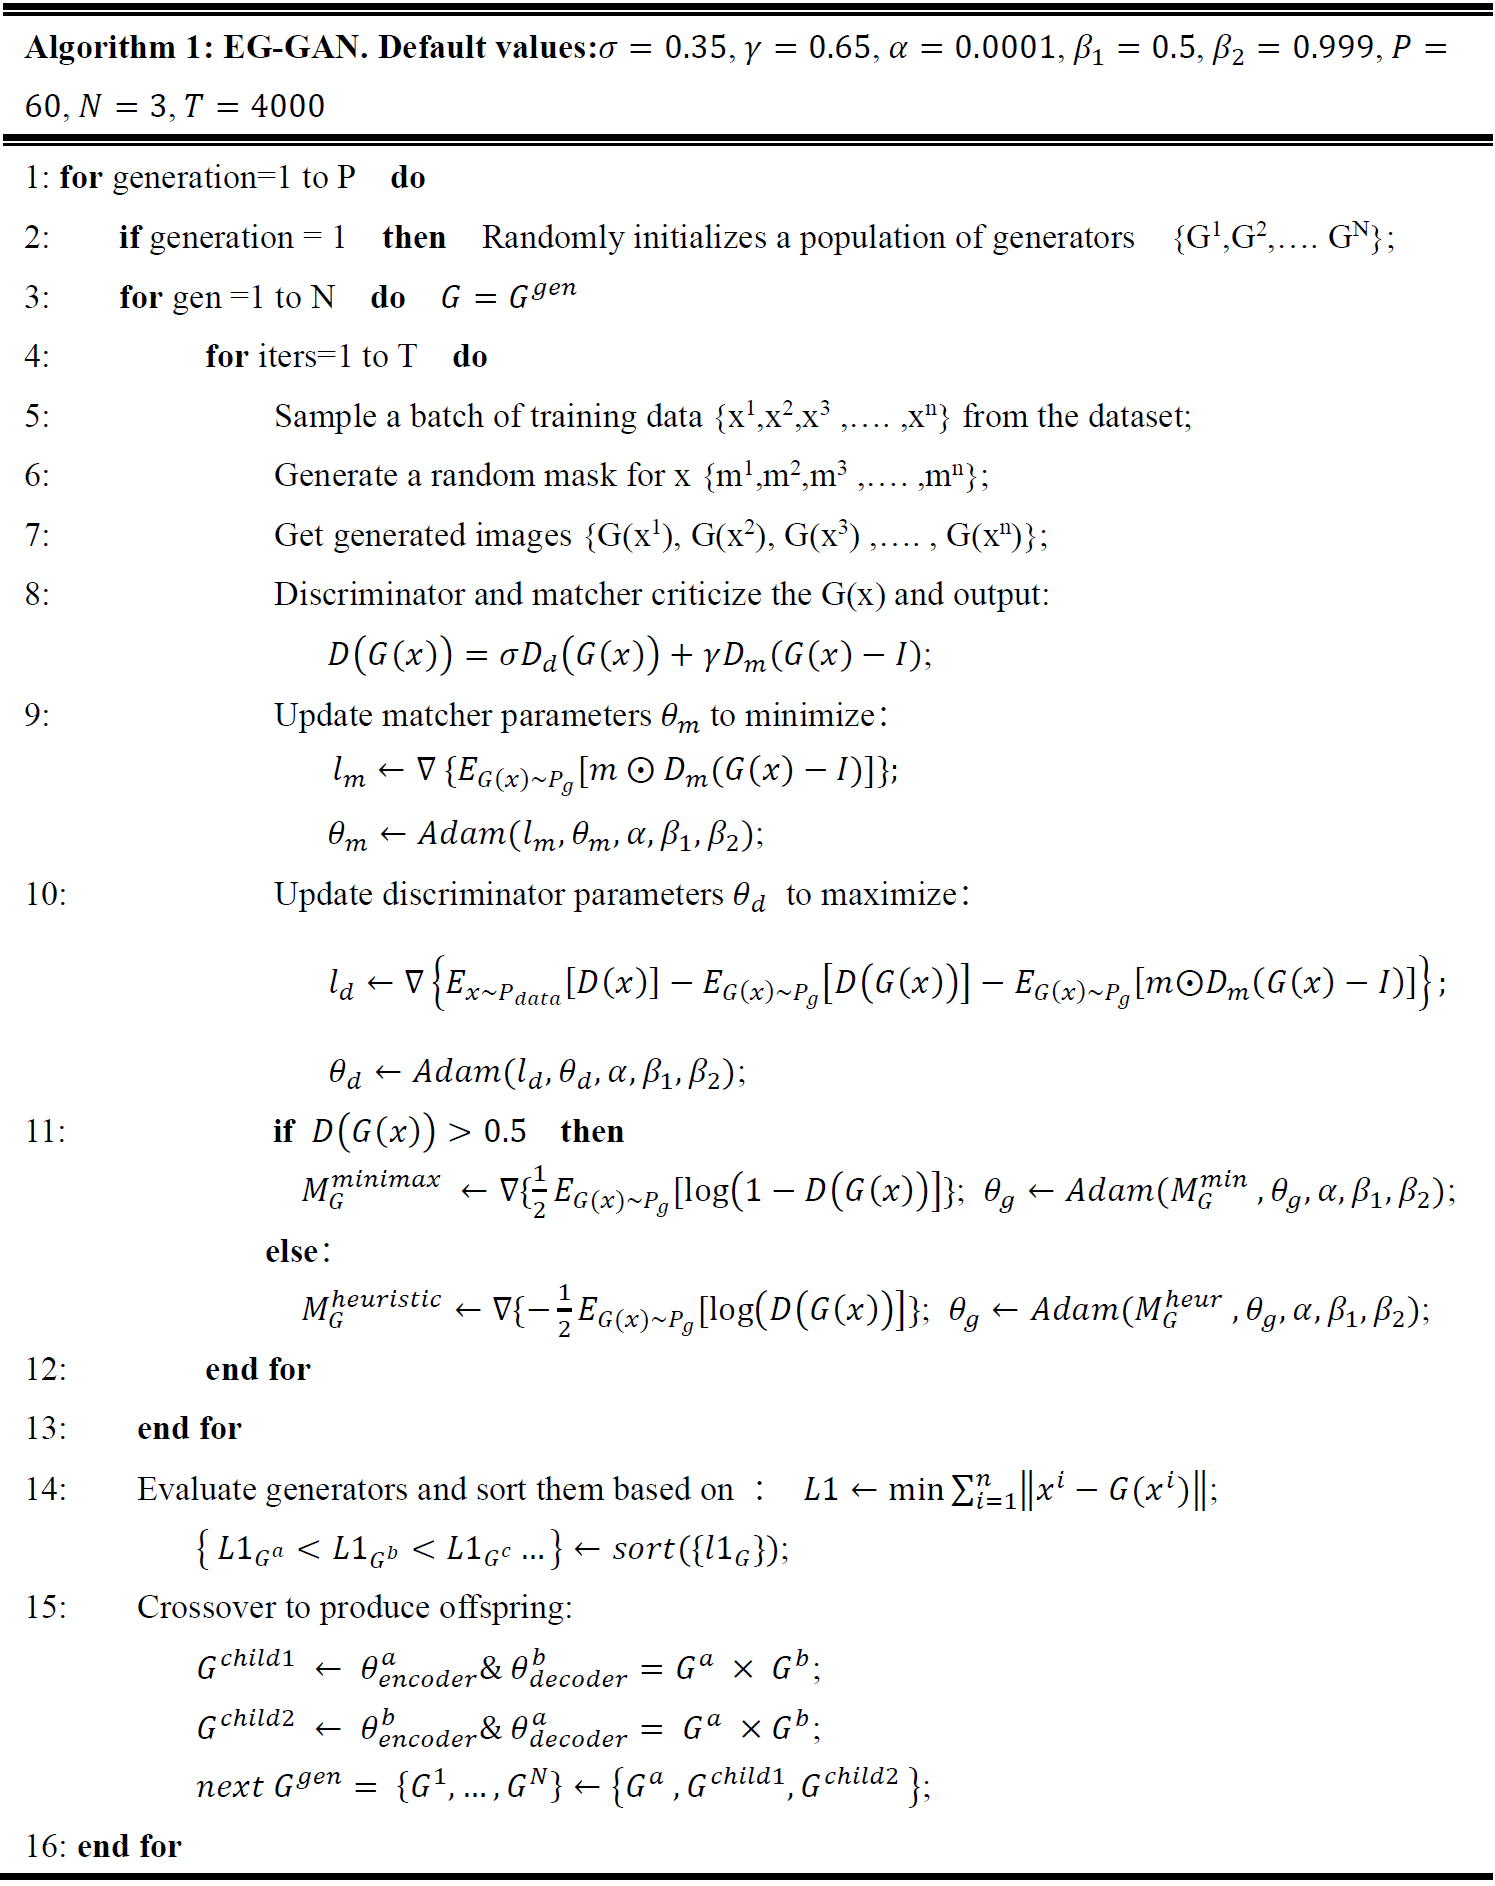
\includegraphics[width=1\linewidth]{figures/Fig3.png}
\caption{EG-GAN Algorithm: P is the number of evolutionary generation, N is the number of generators in each generation, and T is the iteration of mutation. When the hardware permits, N can be expanded appropriately. Simultaneously, to keep N the same during the evolution process, the parent individual can be reserved to the next generation.}
\label{fig:Fig3}
\end{figure}

\section{Experiments}
In the experiment, we use CelebA-HQ\cite{karras2017progressive} as the training dataset. CelebA-HQ is a high-definition human face dataset generated by Nvidia in 2018, which can increase the pixels of images in CelebA\cite{liu2015deep} up to 1024*1024. The pixel size of the face image used in our experiment is 256 * 256, the training set contains 24102 images, and the test set contains 2942 images. Two GTX 1080 Ti GPUs run simultaneously, completing the 60 generations evolution. In our experiments, apart from the inpainting results, we also utilize the PSNR and SSMI indexes\cite{ledig2017photo} to estimate our model.
    \subsection{Ablation Experiment}
    In order to prove the effectiveness of introducing evolution and matcher, the face image is restored by four different settings of our model. For M1, we introduce a reconstruction loss l$_{d}$ to the discriminator and only the heuristic mutation is introduced to the generator. For M2, based on M1, the minimax mutation is added to the generator, thus the generator is optimized by these two mutations. For M3, based on M2, we introduce the matcher and its loss function l$_{m}$ to the whole network to further optimize the discriminator. For M4, based on M3, we introduce evolutionary optimization to the generator, which is the proposed method EG-GAN. Fig.4 shows the ablation results, and Tab1 shows the PSNR and SSIM results under each setting.
    \begin{figure}[htbp]
       \centering
       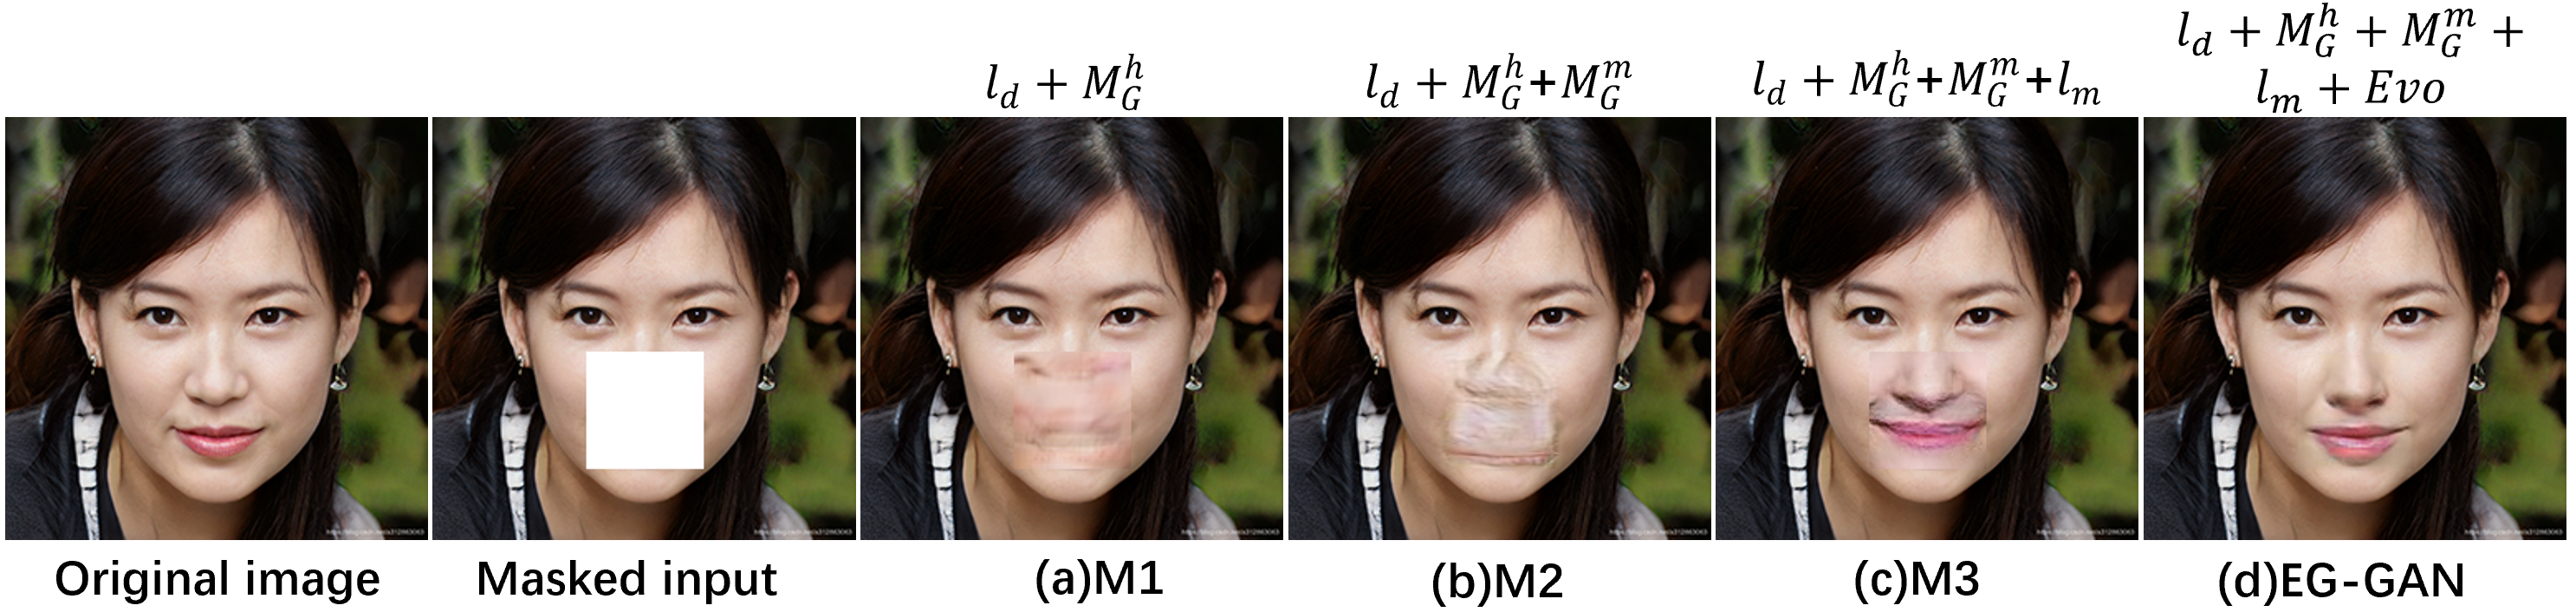
\includegraphics[width=0.8\linewidth]{figures/Fig4.png}
       \caption{Ablation results under different settings}
       \label{fig:Fig4}
    \end{figure}
    \begin{table}[htbp]
    \caption{Quantitative evaluations in terms of PSNR and SSMI under different settings}
	\centering
        \renewcommand{\arraystretch}{1.5}
        \begin{tabular}{|c|c|c|c|c|}
        \hline
        M&M1&M2&M3&EG-GAN\\
        \hline
        SSIM&0.900941&0.913659&0.923995&0.949266\\
        \hline
        PSNR&25.50357&26.68998&29.37788&34.16005\\
        \hline
        \end{tabular}
    \end{table}

    According to the comparison of the results, M1 and M2 can not generate reasonable and clear results, which may be due to model collapse or gradient vanishing problem, as can be seen in Fig4.(a)(b). When the matcher is added, the model can generate a reasonable result in the missing region, but the generated image is a little unclear, and there is an unnatural color transition at the boundary of the missing region, as shown in Fig4.(c). In Fig4.(d), based on the evolutionary selection, EG-GAN can generate more clear inpainting results and get the highest score on SSIM and PSNR .
    \subsection{Evolutionary Process}
    The image inpainting results are generated by the corresponding generators from the 10th to 60th generation, as shown in Fig5.(a). In addition, the performance of EG-GAN can be reflected by the change of L1loss and the M$_{G}$ in Fig5.(b). After the 10th, the downward of L1loss tends to be stable. Because the generated image must have a certain error compared with the original image, which indirectly reflects whether the generator is creative or not. Secondly, based on the M$_{G}$, we can infer the value of D(G(x)), because the generator chooses minimax mutation or heuristic mutation as the loss function of the generator depending on D(G(x)).As shown in Fig.1, we can see that when M$_{G}$ vibrates between 0.5 and -0.25, the corresponding value of D(G(x)) vibrates around 0.5. In Fig5(b), we can see that M$_{G}$ is basically maintained at 0.5 to -0.25 after the 10th generation, indicating that gradient vanishing can be avoided during training.
    \begin{figure}[H]
       \centering
       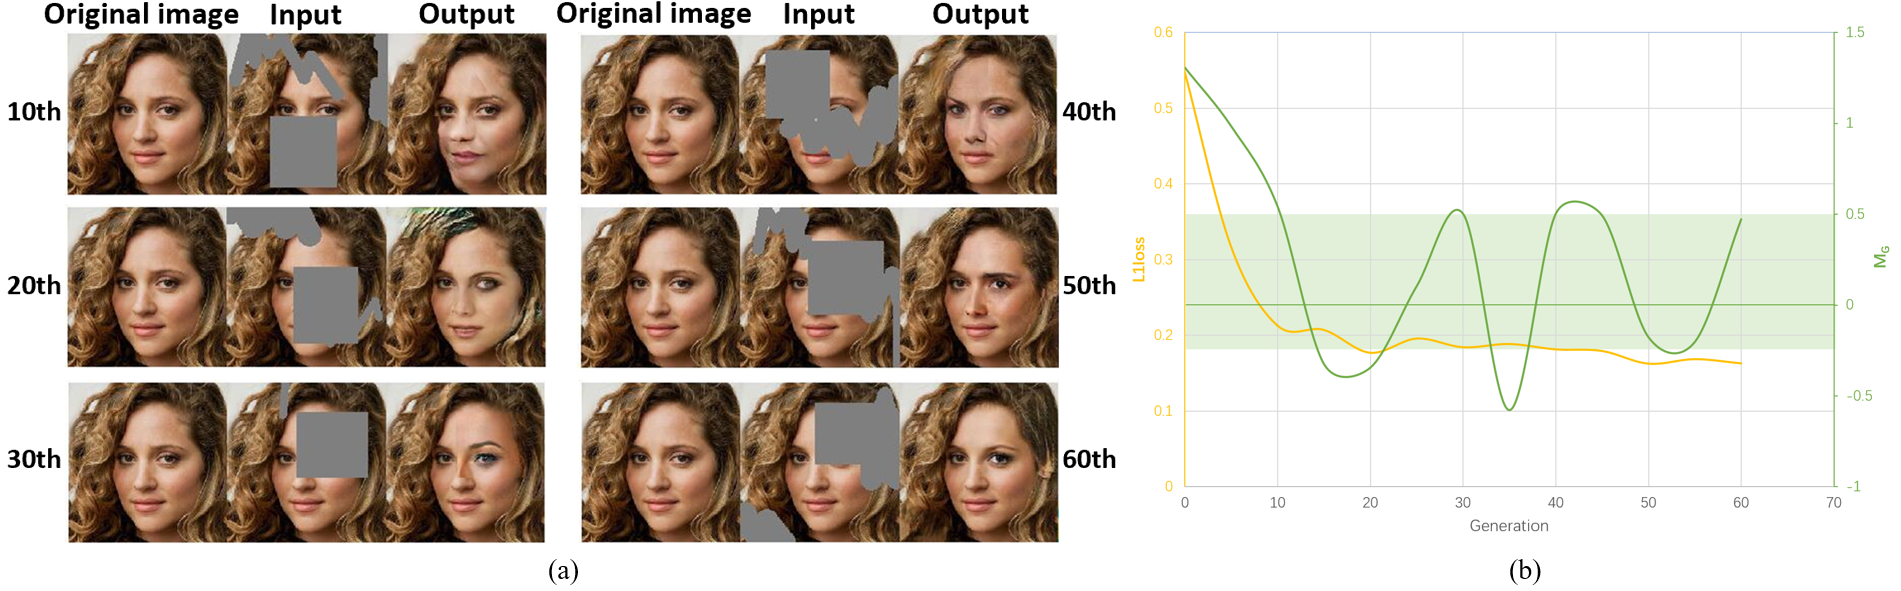
\includegraphics[width=1\linewidth]{figures/Fig5.png}
       \caption{The image inpainting results from different generations(a); L1loss and M$_{G}$ change with generations(b)}
       \label{fig:Fig5}
    \end{figure}
    \subsection{Face Inpainting Results}
    In order to study the influence of different mask sizes on inpainting results, we input eight different square masks into the EG-GAN, and eight masks are numbered from 1 to 8, in Fig6.(a). To a certain extent, SSIM and PSNR decrease as the size of mask increases, as shown in Fig6.(b). However, the downward of SSIM is not as obvious as PSNR. Thus, even if EG-GAN can not achieve high performance in pixel level for larger mask, it can achieve a higher structural restoration. We also did an experiment using a face with glasses, as shown in Fig7.(a)(b)(c).Meanwhile, to test the generalization ability of EG-GAN, we select some images from other datasets, as shown in Fig7.(d)(e)(f). All of these results show that EG-GAN is creative enough to generate images distinctive from the training set, which is significant to avoid model collapse.
    \begin{figure}[H]
       \centering
       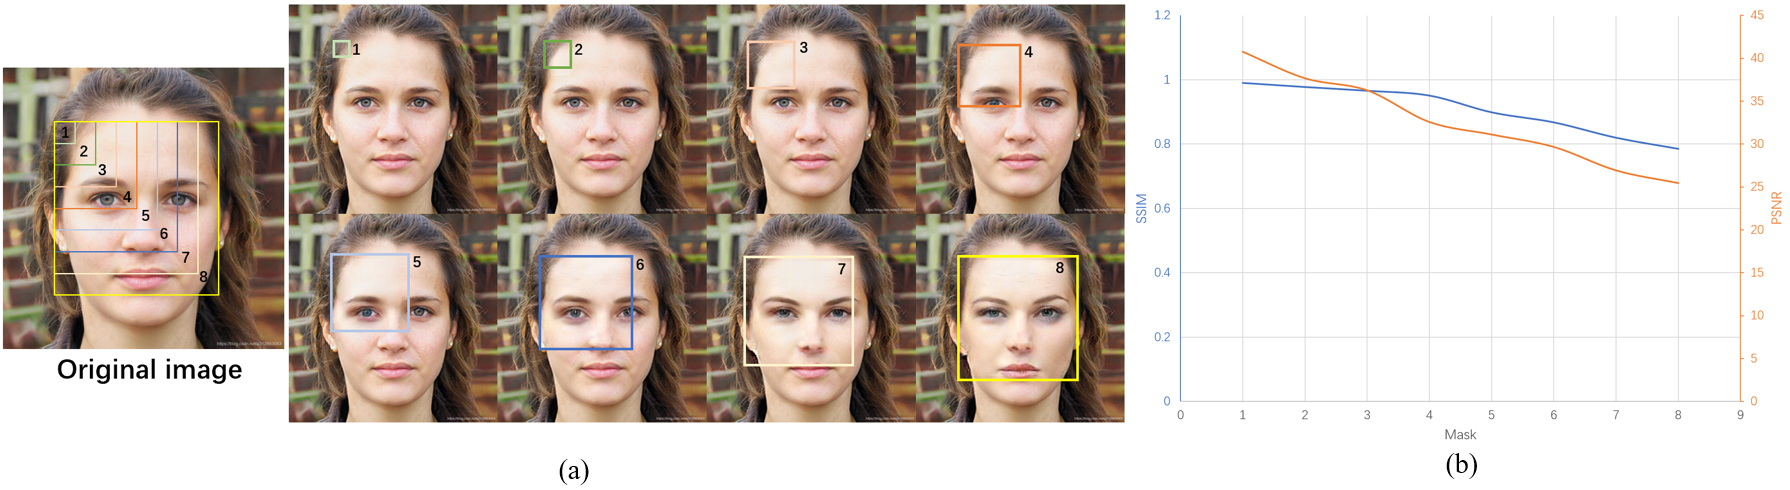
\includegraphics[width=0.9\linewidth]{figures/Fig6.png}
       \caption{Inpainting results of different square mask sizes(a): For mask from 1 to 6 which do not cover the eyes or only cover one eye, EG-GAN can restore image by learning the symmetry of the face. Thus, the inpainting results are very similar to the original image. For mask7 and mask8, it shows that EG-GAN has creative imagination. SSIM and PSNR evaluations at different square mask sizes(b)}
       \label{fig:Fig6}
    \end{figure}

    \begin{figure}[htbp]
       \centering
       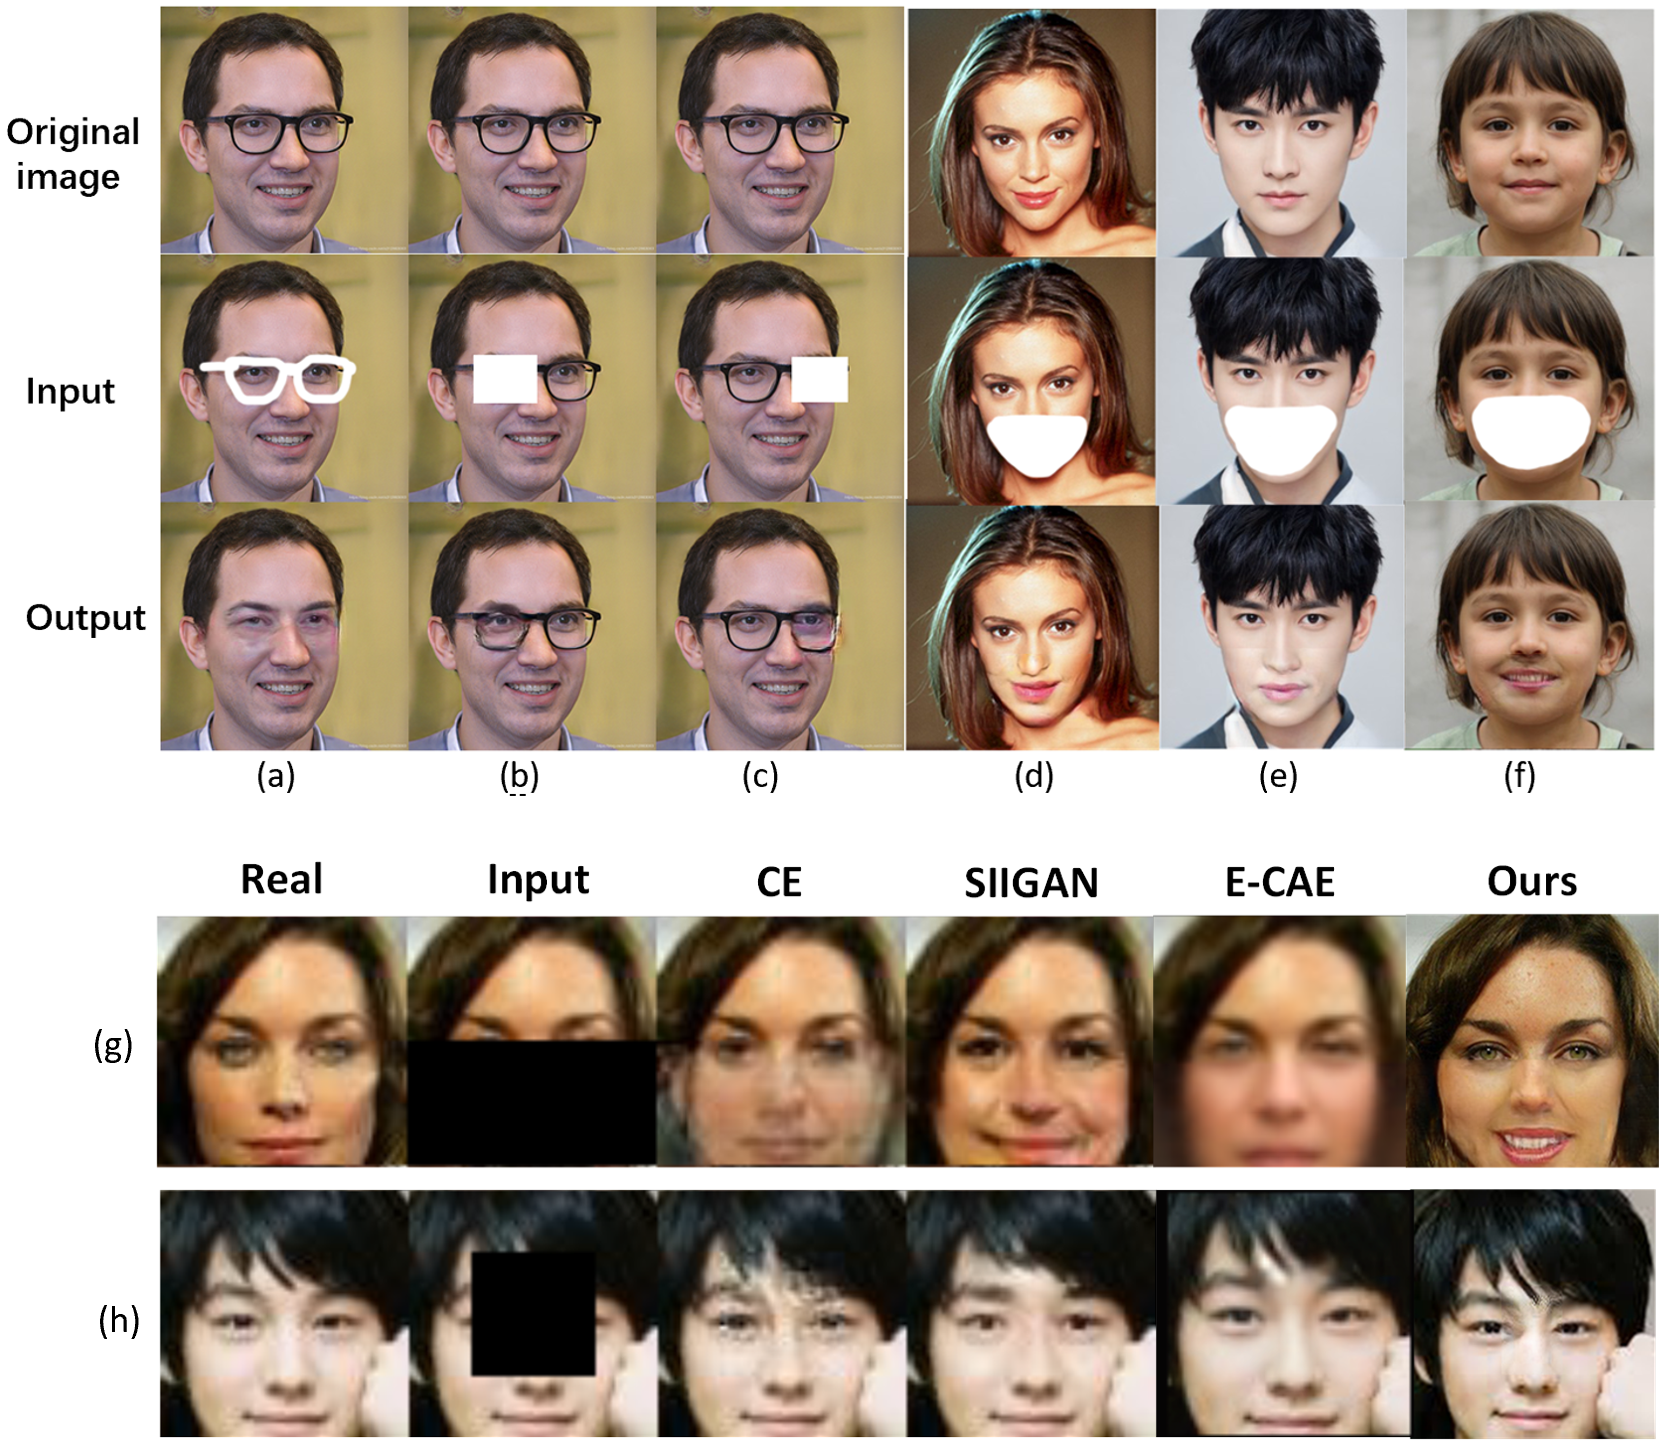
\includegraphics[width=0.7\linewidth]{figures/Fig7.png}
       \caption{Inpainting results of a face with glasses(a)(b)(c): (a):EG-GAN can restore an irregular mask well; (b)(c):It can prove the restoration capability of EG-GAN in both left and right sides. Inpainting results on PubFig dataset\cite{setty2013indian}(d). Inpainting results on non-real face dataset generated by StyleGAN\cite{karras2019style}(e)(f). Image inpainting results of each model(g)(h)}
       \label{fig:Fig7}
    \end{figure}

    Finally, we compare the EG-GAN model with several image inpainting models (CE, SIIGAN, E-CAE), as shown in the Fig7.(g)(h). In the Tab2, the PSNR and SSMI of each model tested on half of the missing image.
    \begin{table}[H]
    \caption{Quantitative evaluations in terms of PSNR and SSMI on different models}
	\centering
        \renewcommand{\arraystretch}{1.25}
        \begin{tabular}{|c|c|c|c|}
        \hline
        Dataset&Models&PSNR&SSMI\\
        \hline
        \multirow{4}{*}{CelebA(half)}&CE&15.5&0.747\\
        \cline{2-4}
        &SIIGAN&13.7&0.582\\
        \cline{2-4}
        &ES-GAN&21.1&0.771\\
        \cline{2-4}
        &EG-GAN&24.2&0.832\\
        \hline
        \end{tabular}
    \end{table}

\section{Conclusion}
This letter proposes a face image inpainting model based on neuro-evolution, which regards the generator as an individual in the population. Generators with excellent performance are selected as the parent individuals, and offspring individuals are generated by crossover. The matcher is designed to assist the discriminator to criticize the image. Both qualitative and quantitative experiments show that EG-GAN can restore various kinds of face images with different masks in sizes, positions, and shapes, achieving reasonable and clear inpainting results.
    

\bibliographystyle{IEEEtran}
\bibliography{Bibfile/An_BIB}

\end{document}
